\documentclass[final,hyperref={pdfpagelabels=false}]{beamer}
\mode<presentation>{\usetheme{Lankton}}
  \usepackage{times}
  \usepackage{ragged2e} %% justify the text.
  \usepackage{amsmath,amsthm, amssymb, latexsym}
  \boldmath
  \usepackage[english]{babel}
  \usepackage[latin1]{inputenc}

\usepackage{graphicx}
\graphicspath{{figures/}}

% \usepackage[orientation=portrait,size=custom,width=40,height=80,scale=.6,debug]{beamerposter}
  \usepackage[orientation=portrait,size=a0,scale=1]{beamerposter} %% this can scale the entire poster to make it smaller or bigger.

%-- Header and footer information ----------------------------------
\newcommand{\footleft}{School of Electrical engineeing, the University of Newcastle, Australia}
\newcommand{\footright}{email: mail@mvkonnik.info}
\title{Fantastic Poster About My Research}
\author{Mikhail V. Konnik}
\institute{The University of Newcastle, Australia}
%-------------------------------------------------------------------


%-- Main Document --------------------------------------------------
\begin{document}
\begin{frame}{}

      \begin{block}{Summary}
        This is a poster containing text and other things
        This part is the summary.  People might read this. $\alpha = 1$
      \end{block}
% 
  \begin{columns}[t]
% 
%     %-- Column 1 ---------------------------------------------------
    \begin{column}{0.32\linewidth}

      %-- Block 1-1
      \begin{block}{Summary}
        This is a poster containing text and other things
        This part is the summary.  People might read this
      \end{block}

      %-- Block 1-2
      \begin{block}{Motivation}
        You can make a poster very quickly and easily by cutting and pasting
        the \LaTeX~codes from the paper!
      \end{block}

      %-- Block 1-3
      \begin{block}{Columns}
        The columns will automatically align with each other and try to look
%         as nice as possible.  You may have to add {\tt$\backslash$vspace\{1pt\}}
        commands to adjust the spacing here and there.  Remember that you can
        use positive or negative numbers.
      \end{block}

    \end{column}%1

    %-- Column 2 ---------------------------------------------------
    \begin{column}{0.32\linewidth}

      %-- Block 2-1
      \begin{block}{Lists}
        \begin{itemize}
          \item You can make
          \item lists, that
          \item allow people to see quickly
        \end{itemize}
      \end{block}

      %-- Block 2-2
      \begin{block}{Math}
        Include math within the text is as simple as $1+1=2$.  You can also
        highlight more important equations like this:
        \begin{equation}
          \int_0^1\sin(x)+\cos^2(x)+\alpha x~d\!x
        \end{equation}
      \end{block}

      %-- Block 2-3
      \begin{block}{Pictures}
        \begin{figure}[htb]
          \centering
          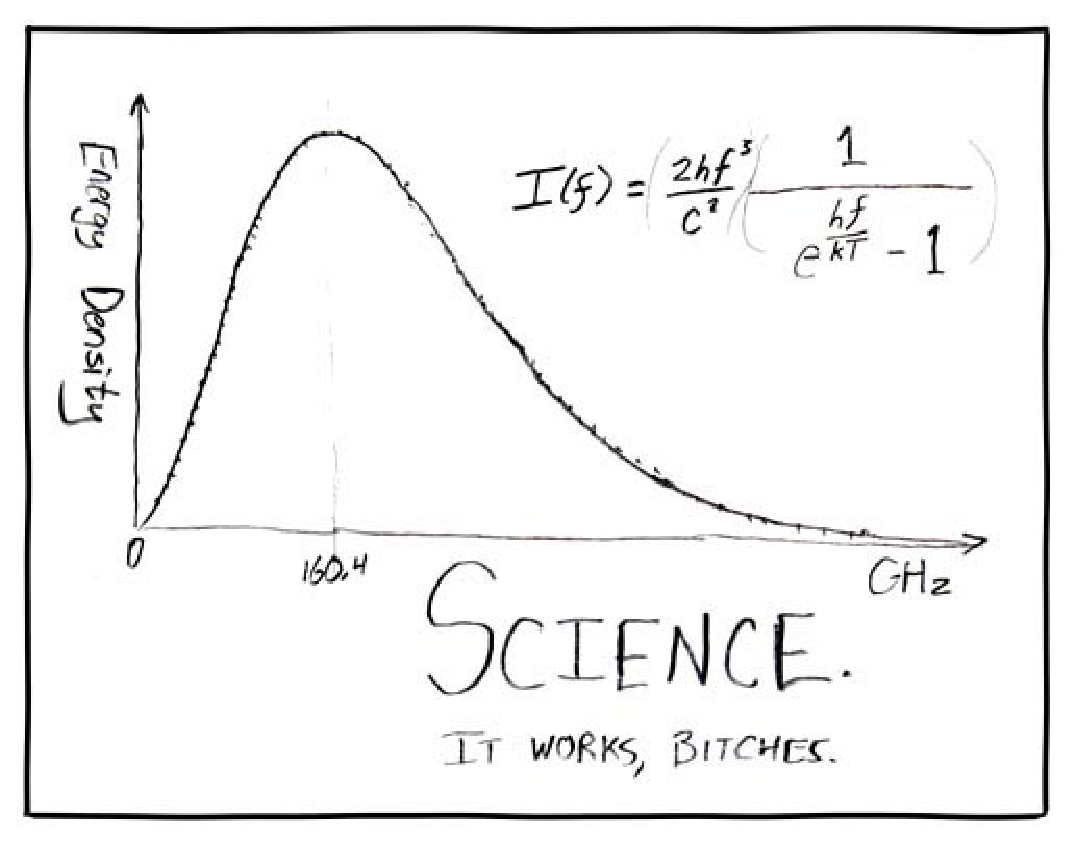
\includegraphics[width=1\columnwidth]{science}
        \end{figure}
      \end{block}

    \end{column}%2

    %-- Column 3 ---------------------------------------------------
    \begin{column}{0.32\linewidth}

      %-- Block 3-1
      \begin{block}{Experiments}
        Remember to put lots of figures on your poster... Nobody reads anymore!
      \end{block}

      %-- Block 3-2
      \begin{block}{Conclusion}
        Much less annoying than PowerPoint.  Copy and Paste from your
        document. Overall, a great idea!
      \end{block}

      %-- Block 3-3
      \begin{block}{Logo}
        To change the logo (if you don't want to represent for Georgia Tech).
        Replace the file {\tt logo.png} and with the logo of your choice!
        Make sure the background is black.
      \end{block}

    \end{column}%3

  \end{columns}

	\begin{block}{Conclusion} \justifying
Adaptive optics is a technique that allows to compensate the impact of atmospheric turbulence in real-time thus improving the quality of astronomical images. Design of the controller is the next stage of this research project.
	\end{block}%-- Block 1-2

\end{frame}
\end{document}